% this file is called up by thesis.tex
% content in this file will be fed into the main document

%: ----------------------- name of chapter  -------------------------
\chapter{Player Engine Design} % top level followed by section, subsection


%: ----------------------- paths to graphics ------------------------

% change according to folder and file names
\ifpdf
    \graphicspath{{X/figures/PNG/}{X/figures/PDF/}{X/figures/}}
\else
    \graphicspath{{X/figures/EPS/}{X/figures/}}
\fi

\section{Overview}
Chapter mainly describe the player engine HCMP Player and its design, usage,
and programming interface. Focus will be on how player engine communicate 
with GUI component, what kind  
``service'' player engine provides. In real implementation, player engine is 
executed in a independent thread, namely perfermer thread. The message queue 
is like unix-style ``pipe'' between 
two programs. The player engine is periodically invoked up by a external timer, 
execute some predefined task. For example, check and message queue and handle 
pending request. The timer period is about 10ms, so any user 
input will immediatelly passed to player engine through message queue and 
be handled, the latency is trivial and can be ignored.

\begin{figure}[H]
\center{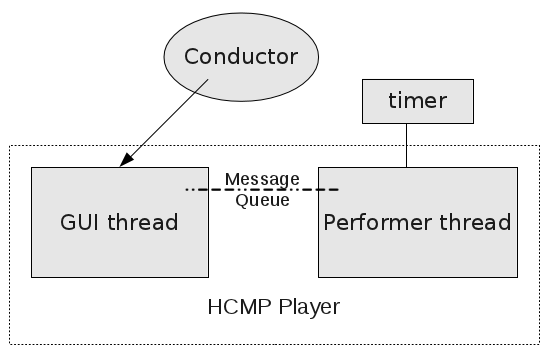
\includegraphics[width=0.55\linewidth]{3/3.png}}
\caption{HCMP GUI Screen Shot}
\label{fig:speciation}
\end{figure}

The player engine server two major purposes, the first purpose is to receive 
message from GUI component and process it, the second purpose is to schedule 
and play midi event at desire time, sometimes, player engine also need to 
reschedule those scheduled events. In concolusion, we can basically divide 
design of player engine  
into two parts, communication and synchronization. Communication refer to the 
way player engine and GUI work together. Synchronization refer to
media synchroization, which involv how schedule midi note, how to resposne to
the change of tempo. 

\section{Communication}

Figure 3.2 illustrate commuication between GUI component and player engine, 
in this figure,  
the GUI component receive request and worked as ``front-end'' part of HCMP Player,
and player engine handle the requeset and worked as the ``back-end'' part. 
In stand-alone mode, the GUI component receive request from  
user-generate events like clicking button or adjustting slider bar. These events are
all captured by GUI component, processed and evnentualy passed to player engine. 
In network mode, the request is captured through network interface, the GUI
is responsible for handle it when request first arrived by network.
Form player engine's perspective, it has no 
idea whether the request is from a user motion or a remote server. 
Based on this scenaio, a unified API between GUI component and player engine is 
defined to
clearly illustrate the responsiblity boundary of each module. Note that the 
API between GUI component and player engine is different from those of network API, 
the former is an internal API between two module, the latter is defined to coordiate
between remote server and multiple instance of HCMP players.

\begin{figure}[H]
\center{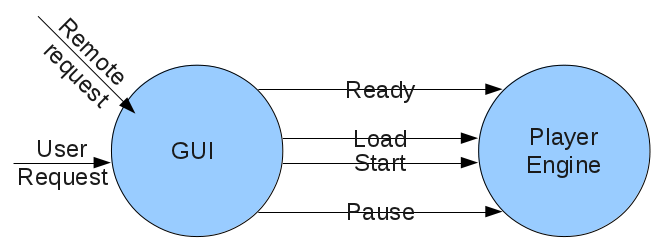
\includegraphics[width=0.7\linewidth]{3/4.png}}
\caption{GUI and Player Engine}
\label{fig:speciation}
\end{figure}

\subsection{Graphic User Interface Thread}

Table 3.2 list the GUI component and its request, in stand-alone 
when user click those  buttons, it will send request to player engine.

\begin{table}[htdp]
\centering
\begin{tabular}{|l||*{2}{c|}}\hline
GUI component & Send Request \\ \hline
load button & load\_file \\\hline
play button & play\\\hline
pause button & pause \\\hline
stop button & stop \\\hline
network button & send\_con\_req \\\hline
tempo slider & change\_tempo \\\hline
volume slider & change\_volume \\\hline
\end{tabular}

\caption[GUI component and request]{GUI component and request}
\label{latexin_genes}
\end{table}

\subsection{State Transition Diagram}

Table 3.2 and 3.3 are state transition diagrams for player engine. Column is state, 
Row is method,  each (column, row) pair in table means that, given current state
if we invoke certain method, what player engine state will transit to.

The player engine only receive and accept control messages from GUI component. 
It immediately process the message upon receiving. In real implementation, 
the player engine has a hash like data structure to store all the invoking
methods, the key is a pair of current state and request, the value is method which 
transit the current state to new state, it is quite similar to previous 
state transition diagram. When the player engine thread firstly 
created, it also initialize a timer to periodically invoke itself after
initialization. Note that to avoid dropping request problem from happening, 
we need make sure that all the routinues can be executed and completed within 
bounded time.

\begin{table}[htdp]
\centering
\begin{tabular}{|l||*{6}{c|}}\hline
\backslashbox{State}{Method}
&\makebox load & play & pause & stop \\\hline\hline
uninitialize & ready & undefine & undefine & undefine \\\hline
ready & ready & pause & ready & undefine \\\hline
playing & ready & playing & pause & ready \\\hline
pause & ready & playing & pause & ready  \\\hline
network& con\_ready & undefine & con\_suspend& undefine\\\hline 
\end{tabular}

\caption[Player Engine State Transition Diagram]{Player Engine State Transition Diagram}
\label{latexin_genes}
\end{table}

\begin{table}[htdp]
\centering
\begin{tabular}{|l||*{2}{c|}}\hline
\backslashbox{State}{Method}
&\makebox change\_tempo & change\_volume\\\hline\hline
uninitialize &  undefine & undefine \\\hline
ready & undefine & undefine \\\hline
playing & apply\_change & apply\_change \\\hline
pause  & apply\_change & apply\_change \\\hline
network & undefine & undefine \\\hline 
\end{tabular}
\caption[Player Engine State Transition Diagram]{Player Engine State Transition Diagram}
\label{latexin_genes}
\end{table}
\section{Media Synchronization}

To accurately schedule the midi note and apply to any tempo chage.  The player 
engine requires two scheduler, real-time scheduler and virtual-time scheduler. 
Usually, a computation will perform some action needed at the present time,
followed by the scheduling of the next action. The real-time scheduler’s role 
is to keep track of all pending actions and to invoke them at the proper 
time, thus eliminating the need
for Players to busy wait, poll, or otherwise waste computer cycles to 
ensure that their next computation is performed on time. Virtual-time
scheduler is built upon the
real-time player, in most of popular music, we can treat 
synchronization happened at beat level. The purpose of virtual-time
scheduler is to schedule everything at beat level, and the huge 
advantage is that once tempo changed, either due to internal parameter 
of midi file or external signal, there is no need to reschedule 
everything. With virtual-time scheduler, we only need to rearrage
limited number of midi notes.

\subsection{Tempo Prediction}
Assumming most popular music forms has common structure of
beats and measures across all instruments. Thus time is measured in beats. 
The basis for synchronization is a shared notion of the current beat 
and the current tempo. Beats are represented by a floating point number, 
hence they are continuous rather than
integers or messages such as in MIDI clock messages. Also, rather than update the
beat number at frequent intervals, we use a linear mapping from time to
beat. This mapping is conveniently expressed using three parameters (b0, t0, s):
\begin{equation}
b = b_0 + (t - t_0) * s 
\end{equation}

where tempo $s$ is expressed in beats per second, at some time in the past beat $b_0$
occurred at time $t_0$, the current time is $t$, and the current beat is $b$.

\begin{figure}[H]
\center{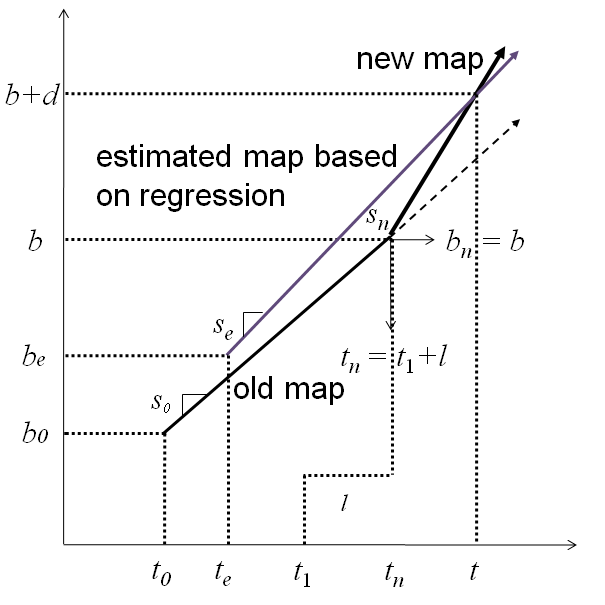
\includegraphics[width=0.5\linewidth]{3/2.png}}
\caption{Midi data display integrated with vitural keyboard}
\label{fig:speciation}
\end{figure}

One advantage of this approach is that it is almost independent of latency.
One can send ($t_0$, $b_0$, $s$) to another computer or process and the mapping will remain
valid regardless of the transmission latency. When parameters change,
there can be a momentary disagreement in the current time among various
processes, but this should be small given that tempo is normally steady.

Media players schedule computation to affect the output at specific beat
times. For example, an audio player may begin a sample playback at beat 3, or a
MIDI player may send a note-on message at beat 5. The current beat time $b$ in 
equation 3.1
refers to the beat position of media which are being output currently.
Since audio output buffer contains 0.01s of audio, then computation associated with
beat b should be performed 0.01s earlier than b. Thus, given a player-specific latency
$l$, we need to compute the real time $t$ at which to schedule a computation associated
with beat $b$. The following formula is easily derived:

\begin{equation}
t = t_0 + (b - b_0) / s - l
\end{equation}

We simply map the beat position $b$ according to ($b_0$, $t_0$, $s$), and then subtract the
latency $l$ to get the computation time $t$.

Our current scheduelr use a simple method to predict the beat . 
Basically, a linear regression over recent taps is used to estimate the
mapping from beat to time. 

Once the tempo and beat phase is established, there is a way to determine
an offset from the arbitrary beat number to the beat number in the score. This might
be determined by a external signal that tells when the system should begin 
to play. The
important point here is that some mechanism estimates a local mapping between
time and beat position, and this mapping is updated as the performance progresses.

\subsection{Scheduling}

Schedulers in the HCMP Player accept requests to perform specific
computations at specific times in the future. Sometimes, the specified time 
can be a ``virtual'' time in units such as beats that are translated to real 
time according to a tempo, as in equation 3.2. An important idea is
that all pending events can be sorted according to beat time 
and everytime the player engine just pick up the earliest event and check its 
time-stamp. If the tempo changes, only the time of this
earliest event needs to be recomputed. When event times are
computed according to equation 3.2, the earliest pending event can change when tempo
changes. 

\section{Player Engine Programming Interface}
In this section, I list all the API that GUI used to communicate with player 
engine. The GUI and player communicate with each other using strings and 
all the parameters are also of type string. A typical string message will be 
like, \texttt{"method\_name;argument1;argument2;argument3"}, each argument is 
separated by a \texttt{";"}
character,. When passing in the parameter string, the player engine
use a \texttt{split}-like function to parse the string and store all elments 
into an array. After parsing the request string, the first element (the request name) 
together with player engine current state form a pair argument. This pair 
will be used as a argument to state transition matrix, then fetch the method, which
transit the current state to a new state.
These API maybe different
from the those APIs defined in next chapter, while most of them has quite similar 
function, the only different lies in that these APIs are defined only for the 
communication purpose of GUI and palyer engine \\
Player control related APIs 
\begin{itemize}
  \item \texttt{load - "load;file\_path"}
  \item \texttt{play - "play;void"}  
  \item \texttt{pause - "pause;void"}
  \item \texttt{stop - "stop;void"}
\end{itemize}
Audio control related APIs
\begin{itemize}
  \item \texttt{change\_volume - "change\_volume;track\_num;velocity"}  
  \item \texttt{change\_tempo - "change\_tempo;tempo\_scale\_coefficient"}  
\end{itemize}
Connection mode related APIs, detail define in following chapter.
\begin{itemize}
  \item \texttt{ini\_connection - "ini\_connection;void"}  
\end{itemize}
